\documentclass[twocolumn]{article}

% Include packages and document structure

\usepackage[utf8]{inputenc}
\usepackage[a4paper,
            bindingoffset=0.2cm,
            left=1cm,
            right=1cm,
            top=1cm,
            bottom=2cm,
            footskip=1cm]{geometry}

\usepackage{lipsum}
\usepackage[english]{babel}



\usepackage{graphicx} % Required to include images
\usepackage[labelfont=sc]{caption} %DT$18/02/2021 caption style
\usepackage{float} %DT$03/01/2020 better image positioning
\usepackage{cuted} %DT$29/07/2022 allows writing over the whole page

\usepackage{braket} % DT$13/11/2021 qm symbols
\usepackage{enumerate} % Custom item numbers for enumerations
\usepackage{placeins} %DT$04/01/2020 \FloatBarrier 
\usepackage{color} % Required for custom colors
\usepackage{amsmath,amsfonts,stmaryrd,amssymb,theorem} % Math packages
\usepackage{siunitx} %DT$03/01/2021 symbols ex:\SI{50}{\micro\second}
\sisetup{range-phrase={\text{\ -\ }},
     input-decimal-markers={.}, 
     range-units = single,
     output-decimal-marker = {.},
     group-digits=false}

\usepackage{booktabs}

\newcommand{\reffig}[1]{Figure~\ref{#1}}
\newcommand{\reftab}[1]{Table~\ref{#1}}
\newcommand{\refeqn}[1]{Equation~\ref{#1}}
\NewDocumentCommand\mat{mmmm}{%
\text{$\begin{pmatrix}#1 & #2\\#3 & #4\end{pmatrix}$}%
}

%%%%%%%%%%%%%%%%%%%%%%%%%%%%%%%%%%%%%%%%%%%% COMMENTS COLORS %%%%%%%%%%%%%%%%%%%%%%%%%%%%%%%%%%%%%%%%
\usepackage{dsfont}
\usepackage{xcolor}
\usepackage{todonotes}
\usepackage{ulem}
\usepackage{listings}

% global

\definecolor{todoxcolor}{HTML}{11aa00}
\newcommand{\todox}[2]{{\color{todoxcolor}\sout{#1}#2}}
\renewcommand{\todox}[1]{\todo[color=todoxcolor!20, inline]{{\it TODO:} #1}}

\definecolor{UniPDcolor}{HTML}{9B0014}
\newcommand{\UniPD}[1]{\todo[color=UniPDcolor, inline]{{\color{white}{\it UniPD contribution:} #1}}}
\newcommand{\todoUPD}[1]{\todo[color=UniPDcolor!20, inline]{{\it TODO UniPD:} #1}}


% people

\definecolor{fedecolor}{HTML}{FEDEBE}
\definecolor{fedecolor2}{HTML}{ff7600}
\newcommand{\fede}[2]{{\color{fedecolor2}{(Fede:\sout{#1} #2})}}
\newcommand{\fedecom}[1]{\todo[color=fedecolor!40, inline]{{\it Fede:} #1}}

\definecolor{blond}{rgb}{0.98, 0.94, 0.75}


%%%%%%%%%%%%%%%%%%%%%%%%%%%%%%%%%%%%%%%%%
%               HEADER
%%%%%%%%%%%%%%%%%%%%%%%%%%%%%%%%%%%%%%%%%
\title{
    \vspace{-1cm}
    
\includegraphics[height=2.5cm]{images/logo_unipd.png}
    \par
    \vspace{0.5cm}
    \textbf{TikTok's Users Analysis in the Context of US Politics}\\
    Advanced Topics in Computer and Networks Security
}
\author{
    Author: {Marco Bellò} \\
    Author: {Alberto Morini} \\
    Supervisor: {Alessandro Galeazzi}
}

\date{18/06/2024}

% Document begin
\begin{document}

\maketitle

%%%%%%%%%%%%%%%%%%%%%%%%%%%%%%%%%%%%%%%%%
%                 BODY
%%%%%%%%%%%%%%%%%%%%%%%%%%%%%%%%%%%%%%%%%

%\section{Intro}
\lipsum
%\input{sections/goals}
%\input{sections/methodology}
%\input{sections/results}
%\section{Extensions}

Regarding echo chambers, privacy inference, engagement, and content impact, better results could be achieved by significantly increasing the number of gathered data points. For example, one could circumvent the limitations imposed by TikTok's APIs by using third-party alternatives such as \url{https://github.com/davidteather/TikTok-Api}.

Another approach to enhance the social graph could involve collecting not only the super-users' followers but also the accounts they follow. This strategy, while powerful, would exponentially increase the number of data points, potentially making the processing phase rather computationally onerous.

Incorporating users' comments into the dataset would allow for sentiment analysis using large language models (LLMs), facilitating the study of polarization. These observations could be intersected with prior findings. Additionally, utilizing language recognition tools and analyzing users' pinned, shared, and liked videos (obtainable through official APIs) could help infer geo-location information, which would be valuable in our geopolitical context.
\begin{abstract}
    \textbf{TikTok has become a dominant social network, and this work studies how users interact on the platform and with each other. This is achieved by creating a social network graph and studying cosine similarity to confirm the presence of echo chambers. Political orientation of users is inferred based on who they follow. Finally, the impact a viral video has on the number of followers is presented, and user engagement is analyzed and visualized.
    }
\end{abstract}

\section*{Introduction}

TikTok is one of the most prominent social networks currently available, boasting over 100 million users in the USA alone \cite{tktkStat}. Approximately 60\% of young adults (aged 18-24) and nearly all children (aged 5-15) use TikTok daily \cite{https://doi.org/10.1002/poi3.287}. This significant influence attracts not only advertisers but also politicians: the Democratic Party began organizing paid influencers as early as the 2020 United States election (for instance, presidential candidate Michael Bloomberg engaged in paid partnerships on social media \cite{10.3389/fcomm.2021.752656}), while Republican and Conservative hype houses campaigned on behalf of political candidates. In Germany, the political party CSU invited influencers to political events and has recently started creating influencer-like social media posts on platforms such as TikTok \cite{10.3389/fcomm.2021.752656}.

This led to the creation of influencer-driven marketing firms, which now claim to control vast, immediately-deployable stables of small-scale influencers for various campaigns. These “nano” and “micro” influencers differ from the conventional image of an influencer: they are everyday people with captive, intimate social media audiences who represent demographics particularly appealing to U.S. political campaigns, such as Latinos in South Florida, Black voters in Atlanta, and college-educated women in the Rust Belt \cite{theHilltktk}. Political influencers often do not have an institutional background, in fact most of the times their notoriety and fame is platform-built \cite{doi:10.1177/20563051231177938}.

Despite this political engagement, TikTok has attempted to market itself as a platform for everything but politics: since 2019 the company has banned paid political advertising, stating that “the nature of paid political ads is not something we believe fits the TikTok platform experience.” Nevertheless, many creators regularly use the platform to disseminate political messages and viewpoints without disclosing whether the content is sponsored or not \cite{mozilla,politico}.

Given these dynamics, there is considerable value in studying user interactions on the platform. This work aims to do so, focusing on the context of the 2024 U.S. political elections. The study will examine user movements using a social graph, analyze user similarity through cosine similarity, infer political affinity, measure engagement, and visualize the impact publishing a video has on followers and comments.
\section{Data Gathering}

Considering the context (US elections) it is imperative to have users' data divided between left and right-leaning, so a group of \textit{super-users} was selected using various sources. 
\textit{Super-users} are defined as follows:

\begin{itemize}
    \item Influencers: people whose notoriety is platform-built, without a background in institutions of entertainment;
    \item Politicians;
    \item Newspapers or news sites (i.e., The Washington Post).
\end{itemize}

The complete followers list, with relative sources (missing if selected arbitrarily by the authors), is as follows:

\begin{itemize}
    \item Left-Wing: 
        \begin{itemize}
            \item @aocinthehouse \cite{wikiDem,yougovDem}
            \item @bernie \cite{wikiDem,yougovDem}
            \item @chrisdmowrey \cite{foxRight}
            \item @cnn \cite{biasCheck1,biasCheck2}
            \item @democracynow.org [unofficial]
            \item @genzforchange \cite{climateCulture}
            \item @ginadivittorio \cite{NYTpayInfluencers}
            \item @harryjsisson \cite{foxRight}
            \item @huffpost \cite{biasCheck1,biasCheck2}
            \item @msnbc \cite{biasCheck1,biasCheck2}
            \item @newyorker \cite{biasCheck1,biasCheck2}
            \item @nytimes \cite{biasCheck1,biasCheck2}
            \item @repbowman \cite{politico}
            \item @rynnstar \cite{https://doi.org/10.1002/poi3.287}
            \item @teamkennedy2024 \cite{wikiDem,yougovDem}
            \item @thedailybeast \cite{biasCheck1,biasCheck2}
            \item @underthedesknews \cite{foxRight}
            \item @vox \cite{biasCheck1,biasCheck2}
            \item @washingtonpost \cite{biasCheck1,biasCheck2}
        \end{itemize}
    \item Right-Wing:
        \begin{itemize}
            \item @alynicolee1126 \cite{mozilla}
            \item @babylonbee \cite{foxProFreeSpech}
            \item @clarksonlawson \cite{foxRight}
            \item @dailymail \cite{biasCheck1,biasCheck2}
            \item @dailywire \cite{biasCheck1,biasCheck2}
            \item @itsthemandrew \cite{mozilla}
            \item @notvictornieves \cite{foxRight}
            \item @real.benshapiro \cite{doi:10.1177/20563051231177938}
            \item @studentsforlife \cite{foxProFreeSpech}
            \item @theisabelbrown \cite{mozilla}
            \item @thesun \cite{biasCheck1,biasCheck2}
        \end{itemize}
\end{itemize}

Due to time and computational constraints, only five super-users had been selected from each group: \textit{@alynicolee1126, @babylonbee, @real.benshapiro, @clarksonlawson, @notvictornieves} for right-leaning, and \textit{@thedailybeast, @huffpost, @aocinthehouse, @repbowman, @newyorker} for left-leaning super-users. \\
All data has been gathered using TikTok's official APIs (\url{https://developers.tiktok.com/doc/overview/})

\subsection{TikTok's APIs}

TikTok's APIs requires prior authentication using a Secret Key and a Client ID, both of which can be obtained by making a personal request to the platform's staff. 
Then, each call to the API must be authenticated with a Bearer token, previously obtained through the appropriate authentication endpoint. Each one has its own query string and body parameters to be included in the HTTP request.

There is a daily limit of 100,000 records (which resets at 12 AM UTC) for videos and comments while, for the followers/following endpoint, the limit is set up to 2 million records (\url{https://developers.tiktok.com/doc/research-api-faq/}).

In this project, every call is parameterized to retrieve the maximum allowed data, typically 100 records. However, the APIs do not always provide the exact data requested, possibly due to a lack of content or other unknown issues.

\subsubsection*{Download Component}

A wrapper for the APIs has been realized for data gathering, which simply makes WebAPI calls and stores the results.
Almost every public endpoint provided has been totally covered by the script, specifically: users' followers, users' videos, videos' comments, following users, liked videos, and users' information.

In the first step, the script authenticates to TikTok's endpoint, gaining the token, which will be refreshed a few minutes before its 2-hour lifespan. Then it starts retrieving the data batch required, storing each response in a JSON file for later analysis.

For the specified number of videos, in this case 100 per month for each super-user (see second code block of section \ref{lst:query}), the script will download their metadata and store them, before concluding its job by retrieving super-users' followers.

\begin{lstlisting}[language=Python]
# @query {JSON} the video query as specified in the TikTok docs
# @nrVideo {int} the number of videos which we want to download
# @startDate {string} in Unix format
# @endDate {string} in Unix format -- NB: can't be greater than a month
# @filename {string} of JSON where data will be stored
def processVideo(query, nrVideo, nrComments, startDate, endDate, filename):
    ....

processVideo(videoQuery,100,200,'20240301','20240330','influencer-month')
\end{lstlisting}

\subsubsection*{Amount of Data Downloaded}

For each video, followers have been downloaded (100 per request) for up to 5 days, within 3-hour intervals, allowing for the retrieval of a theoretical number of followers equal to 4,000:

\[ (100 \text{ users} \times ((24 \text{h}/3 \text{h}) \times 5 = 40 \text{ requests})) = 4000 \]

However, such numbers are reached only if all new followers are distinct in every call, which is difficult to achieve within such a short time span.

Since TikTok's APIs return the user who has started following the influencer from the date (in Unix format) declared in the body of the request (called cursor), the problem of duplicated accounts arises.

To clarify: if \textit{JohnDoe} follows \textit{MrWhite} on 31/12/2023 at 10:00:00 and \textit{MrWhite} does not gain 100 new followers in the next 3 hours, \textit{JohnDoe} will also be included in the request at 31/12/2023 at 13:00:00.

To solve this problem, a Python script (\textit{DataCleaner.py}) was created, which keeps only the first occurrence (sorted by ascending date) of each username found in the total downloaded data.

\begin{lstlisting}[language=Python]
for i in range(0,len(total)-1):
for j in range(i+1, len(total)):
    if(total[i].get("influencer")==total[j].get("influencer")): ##check if the same influencer (we don't want to remove common followers)
        total[i]["followerList"] = [elem for elem in total[i].get("followerList") if elem not in total[j].get("followerList")]
\end{lstlisting}

Additionally, video metadata (such as views, likes, number of comments, etc) and super-users' public information (with a single call for each one) are stored for a later analysis. 

Ultimately, the total amount of data downloaded, divided among 10 super-users, is as follows:
\begin{itemize}
    \item 35,798 distinct followers;
    \item 182 videos.
\end{itemize}
\section{Privacy and Echo Chambers}

To help visualize all the gathered data, identify the presence of echo chambers, and infer the political views of users, super-users' followers were used to create a social network graph and a cosine similarity matrix.

\subsection{Data Preparation}

First, a list of super-users' followers was gathered via TikTok's APIs in the form of a JSON file, and then processed with a script to get the following structure (we can ignore \verb+"videoID"+ and \verb+"videoDate"+):

\begin{lstlisting}[language=json]
[
    {
        "influencer": "ith-super-user Name",
        "videoID": "videoID",
        "videoDate": "videoDate",
        "followerList": [
            "follower1",
            "follower2",
            "follower3",
            "follower4",
            "follower5",
            "follower6",
            "follower-k"
        ]
    }
]
\end{lstlisting}

To clarify, here follows a partition of the real JSON data used:

\begin{lstlisting}[language=json]
    {
        "influencer": "huffpost",
        "videoID": "7354208741996186911",
        "videoDate": "2024-04-05 11:46:08",
        "followerList": [
            "mathieucambet",
            "raphclp",
            "jennet153"
        ]
    },
    {
        "influencer": "huffpost",
        "videoID": "7354208741996186911",
        "videoDate": "2024-04-05 20:46:08",
        "followerList": [
            "doodlegolden0",
            "evanroyalaug",
            "cshanebritt",
            "kabed70"
        ]
    },
\end{lstlisting}

JSON data is then imported to \textit{Social\_Graph.r} for analysis:

\begin{lstlisting}[language=R]
data <- fromJSON(paste(readLines("data.json")))

left_influencer_names <-  # vector of strings with left 
                          # super-user names
right_influencer_names <- # vector of strings with right 
                          # super-user names

# data.frame used to calculate all the graphs and tables
full_total <- data.frame(
  influencer = data$influencer,
  followerList = I(data$followerList)
)

full_influencer_names <- union(left_influencer_names, 
                               right_influencer_names)
\end{lstlisting}

Now we have three data structures to work with: two vectors with all super-users' names and a \verb+data.frame+ that stores all super-users and their gathered followers, as shown below:

\aCapo{}
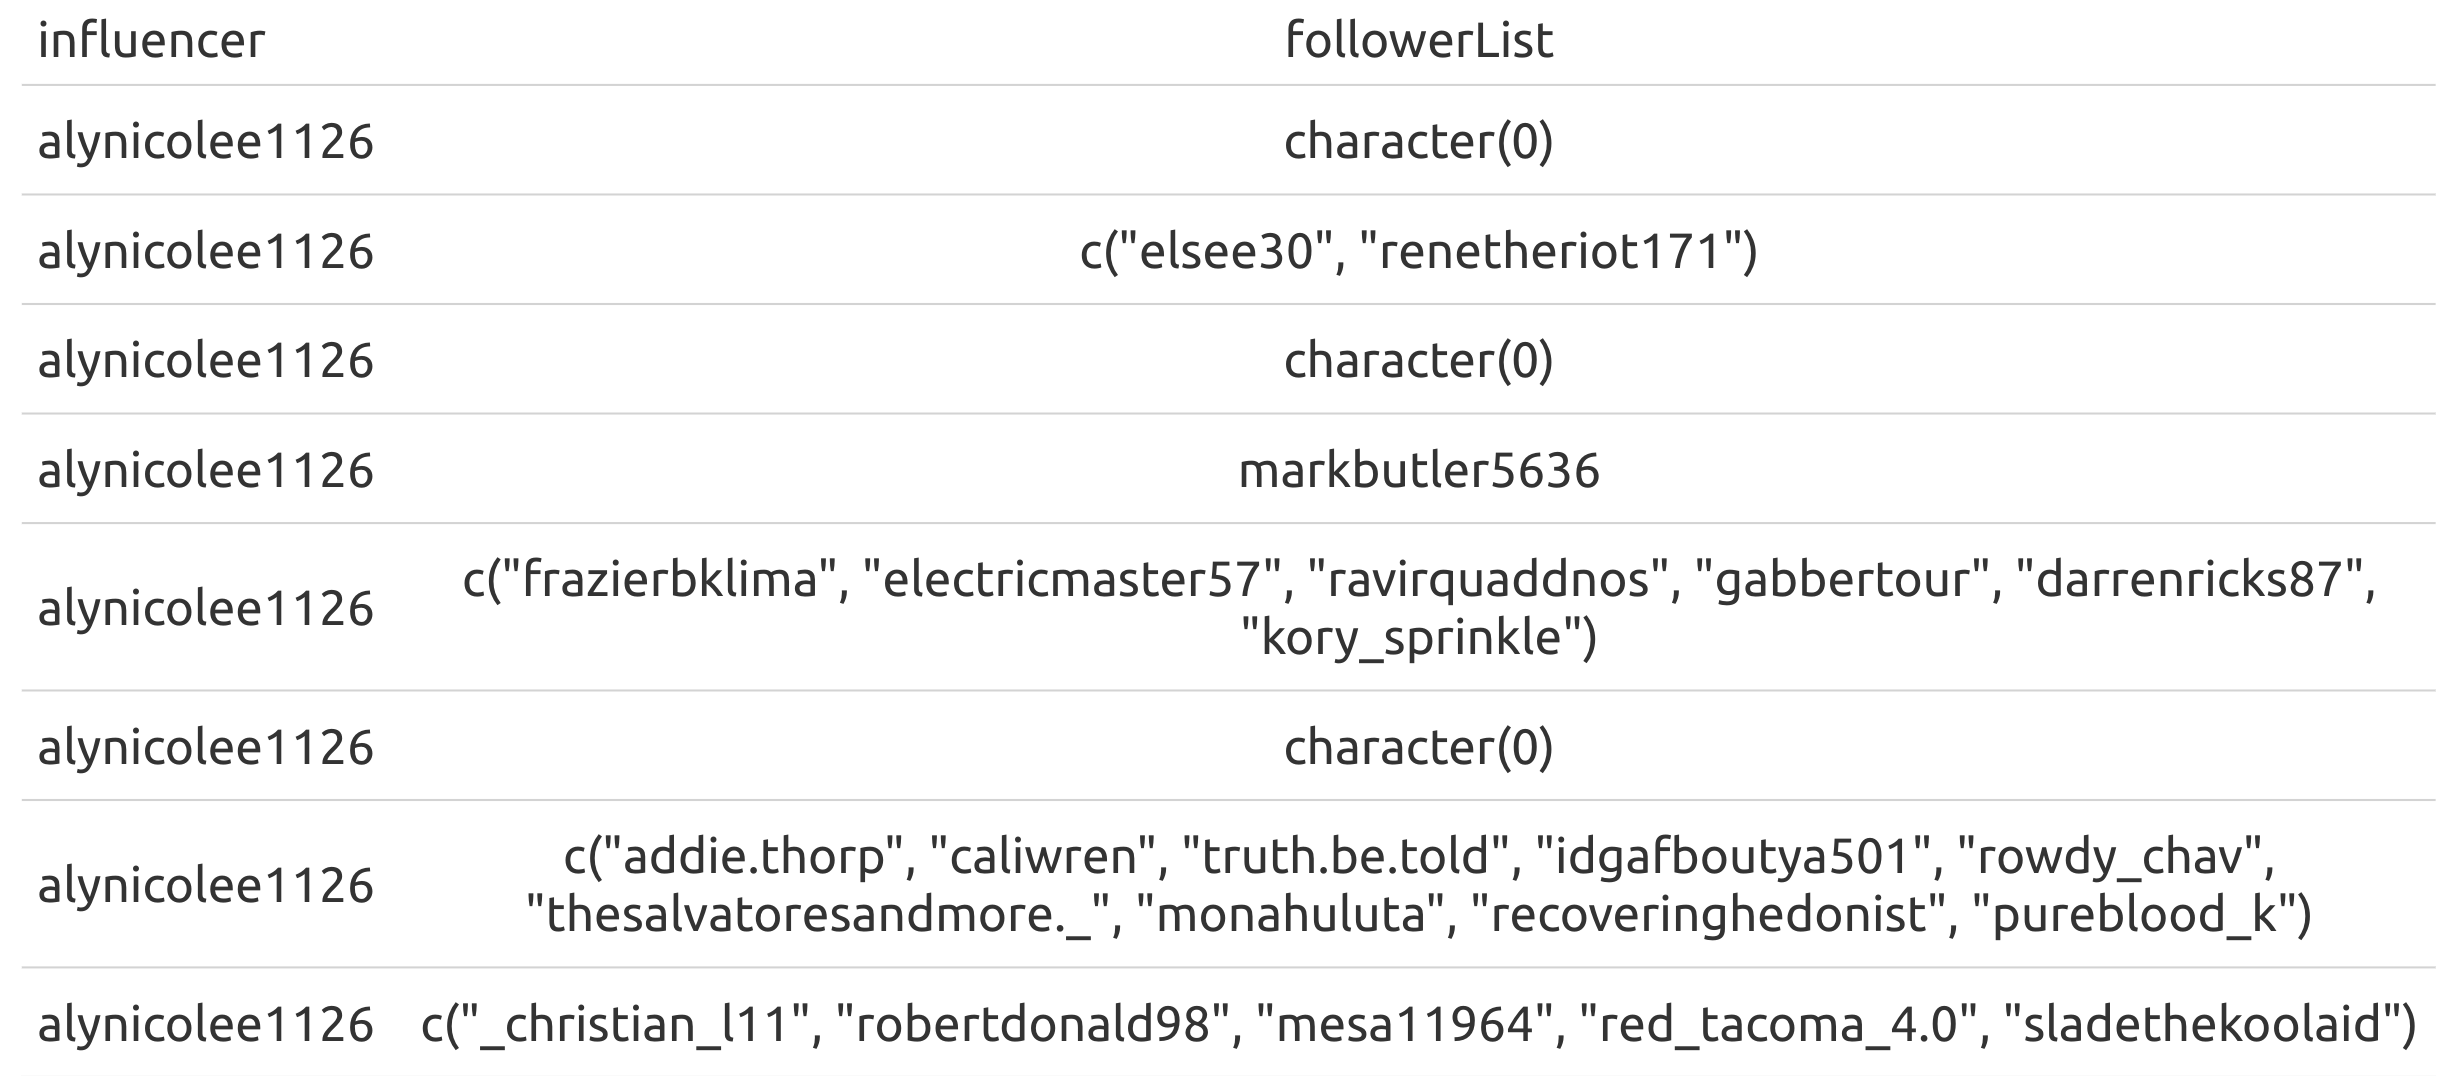
\includegraphics[width = .48\textwidth]{images/total_table_p23.png}

\subsection{Social Graph}

Broadly speaking, a social graph is a graph that represents social relations between entities, were vertices (or nodes) represents users and edges represents relations between such users. It is a model of representation of a social network, and has been referred to as "the global mapping of everybody and how they're related".

To give a brief example: if Alice and Bob are friends on a social network, in a social graph they would be represented each as a node, and there would be an edge between them.

The term was popularized at the Facebook F8 conference on May 24, 2007, when it was used to explain how the newly introduced Facebook Platform would take advantage of the relationships between individuals to offer a richer online experience \cite{wikiSAN}.

\aCapo{}
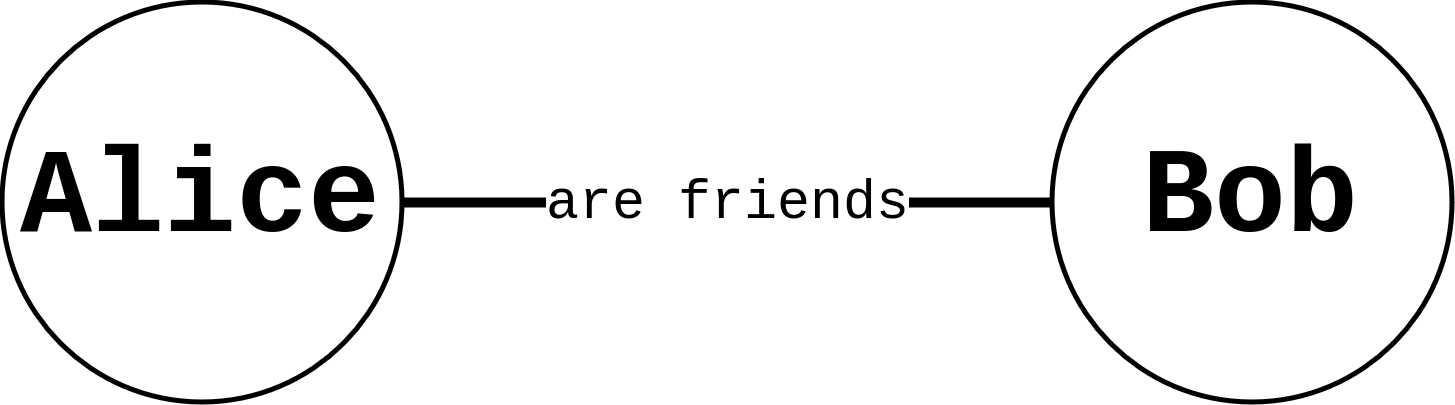
\includegraphics[width = .5\textwidth]{images/alice_bob_san.png}

Employing a social graph has numerous advantages: it helps visualize all gathered data (all users and their relations), identify the presence of echo chambers and provide insights to analyze the network as a whole. \\
The graph that follows clearly demonstrate that, considering the gathered data, users do not interact with each other outside their communities, thus forming cliques that can be interpreted as echo chambers:

\aCapo{}
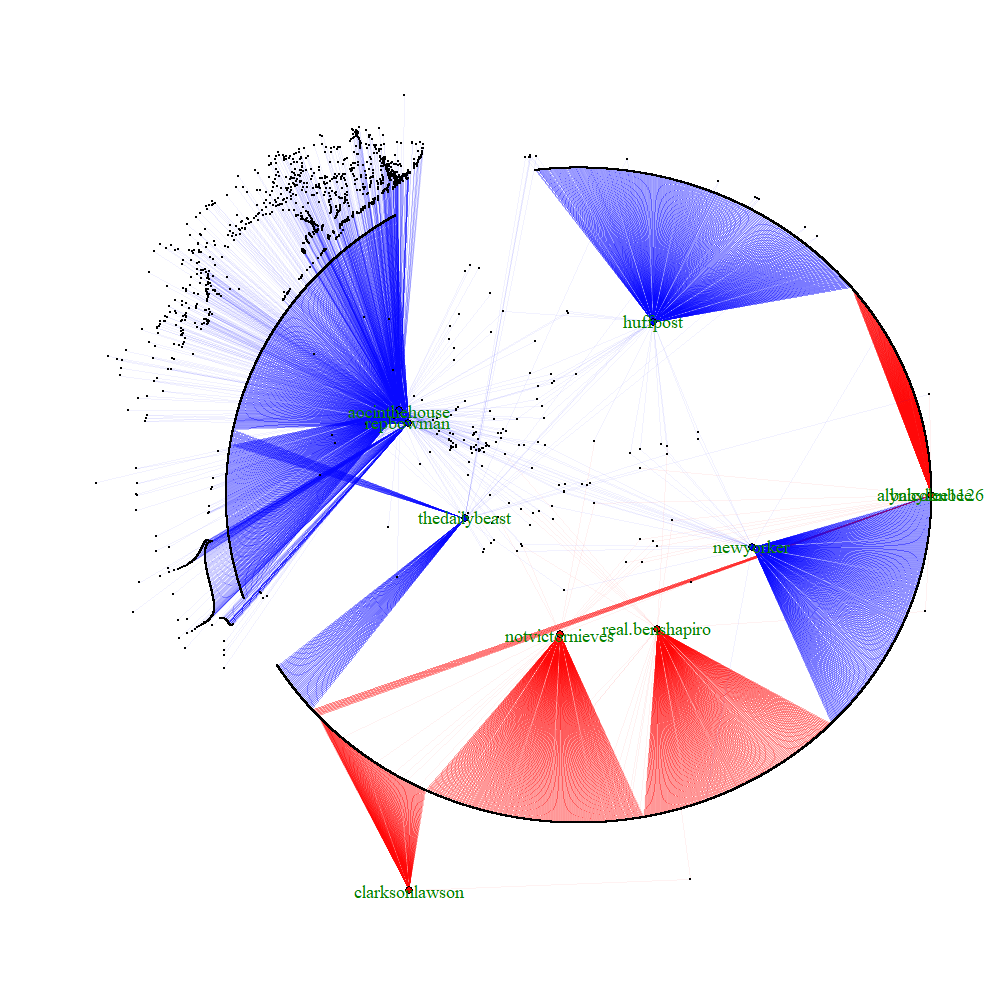
\includegraphics[width = .5\textwidth]{images/final_combined_san_graph.png}

Unfortunately the above graph could be difficult to understand due to the exceptional amount of data points, so here follows a mock-up graph made with a reduced dataset to help clarify how it works:

\aCapo{}
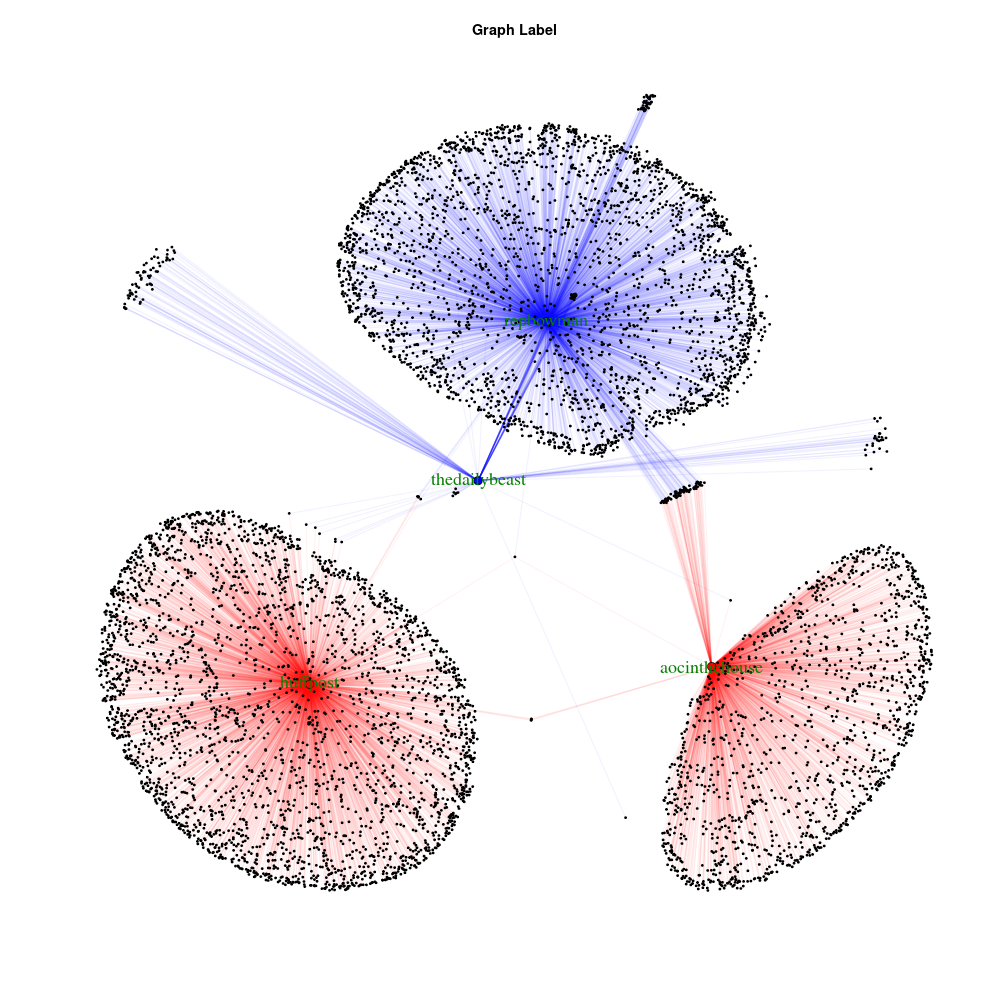
\includegraphics[width = .5\textwidth]{images/mockUP_san.png}

Super-users can be easily identified: their nodes are larger, labeled and, most notably, they are at the center of their respective sub-graphs. 

All black vertices represents followers of the super-users, unlabeled for improved readability, and the edge color represent the political orientation of the super-user they are connected to(red for \textcolor{red}{right-leaning} and blue for \textcolor{blue}{left-leaning} super-users). 

To clarify: if \textit{@user-Alice} follows super-user \textit{@aocinthehouse} (official account of Congress member Alexandria Ocasio-Cortez), which is classified as a left-leaning super-user, the edge connecting them will be blue. 

Conversely, if \textit{@user-Bob} follows super-user \textit{@thesun} (official account of UK's tabloid "The Sun"), which is classified as a right-leaning super-user, the edge connecting them will be red.

\subsection{Cosine Similarity}

Having a graphical representation of a network is valuable: images are easier to recognize, process, and recall. When words enter long-term memory, they do so with a single code. Pictures, on the other hand, contain two codes: one visual and one verbal, each stored in different brain regions (Paivio). The dual-coding nature of images allows two independent ways of accessing visual memories, increasing the odds of remembering at least one. Adding illustrations to text aids comprehension and learning \cite{10.21083/partnership.v10i1.3137}. However, it is also advisable to measure the similarity between users numerically.

Broadly speaking, there are two types of similarity measures between nodes in a network: edge similarity, which provides the index of intersection of parent nodes, and global structure similarity, that aims to evaluate the similarity between two nodes in the context of the whole network. Regarding the latter, Salton Index, Jaccard Index, and Sorensen Index always have good performance, while cosine similarity's computational complexity is very high when applied to large volumes of data \cite{smilarityMeasuresSurvey}. When the data is dense, structure-based indices like Salton's can perform as well as the cosine index but with lower computational complexity. Furthermore, when the data is sparse, structure-based indices outperform the cosine index \cite{10.1016/j.phpro.2010.07.033}.

\aCapo{}
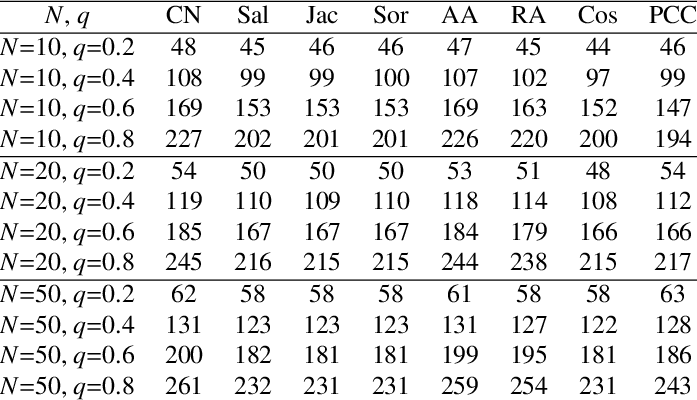
\includegraphics[width = .5\textwidth]{images/salton_precision.png}

The above table shows values regarding precision in inferring similarity between users: Salton index (\textit{Sal} column) seems to perform the best \cite{10.1016/j.phpro.2010.07.033}, therefore it has been used in this work to measure similarity between super-users.

Index formula is as follows: 

$$s_{xy}=\frac{|\Gamma(x)\cap\Gamma(y)|}{\sqrt{k_x\times k_y}}.$$

All index values are calculated for each couple of super-users and shown in the following table where, as mentioned before, blue represent left-leaning and red represent right-leaning super users: 

\aCapo{}
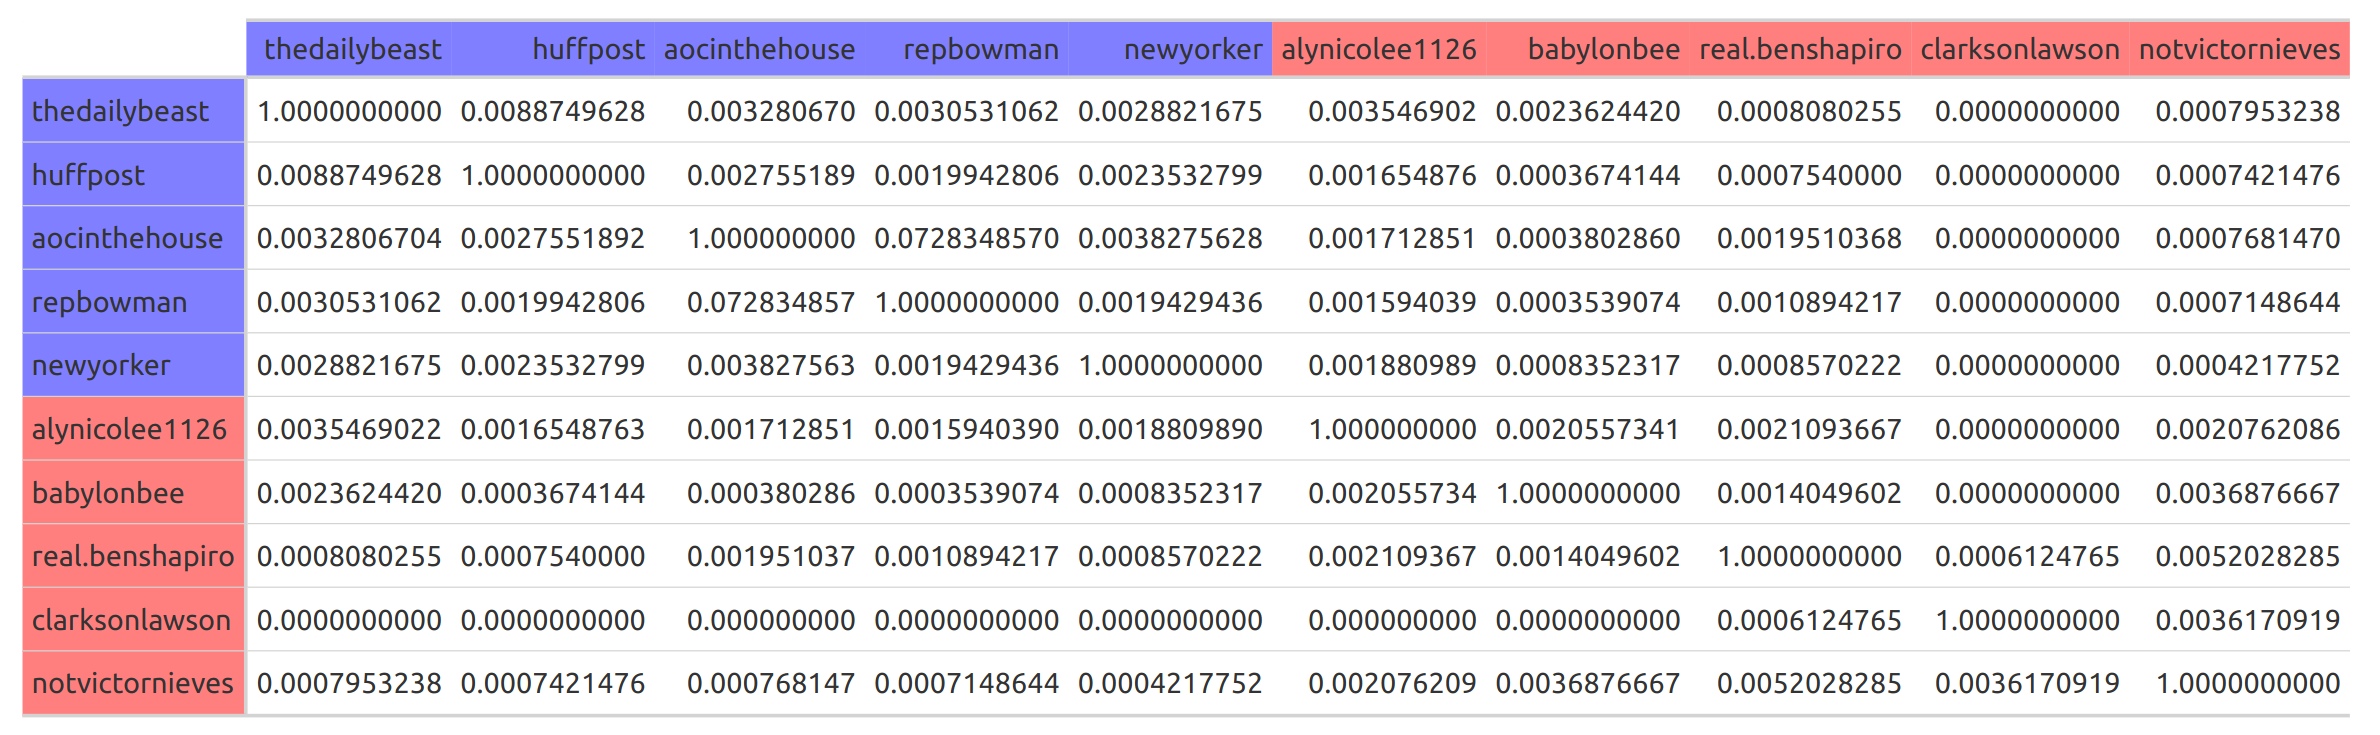
\includegraphics[width = .5\textwidth]{images/final_salton_matrix.png}

Salton index values range between 0 and 1, with the diagonal of the matrix showing all values equal to 1 because a super-user is always identical to itself. The table confirms numerically what could be seen in the social graph: super-users share very few followers, which means that each community is an echo chamber.

\subsection{Privacy Inference}
Another way to leverage social network information, specifically the network structure (edges and their respective nodes), is to infer users' attributes. This falls under classification problems (identifying which of a set of categories an observation belongs to, such as classifying an email as "spam" or "not spam") \cite{wikiClassification}, and such techniques have been employed in this context (e.g., k-nearest neighbors classification \cite{wikiKNN}).

The objective here is to infer the political orientation of users based on the super-users they follow. Given the scarcity of super-users, the presence of only two sets (left and right-leaning), and the high degree of isolation between communities, complex statistical tools are deemed unnecessary. The idea is straightforward: if \textit{user-Alice} follows mainly left-leaning super-users (e.g., \textit{aocinthehouse}, \textit{bernie}, \textit{repbowman}), that user is classified as left-leaning. Conversely, if \textit{user-Bob} follows mainly right-leaning super-users, he is classified as right-leaning.

The following table shows users following more than one super-user from both lists of left and right-leaning super-users, with results ordered by the number of super-users followed.

\aCapo{}
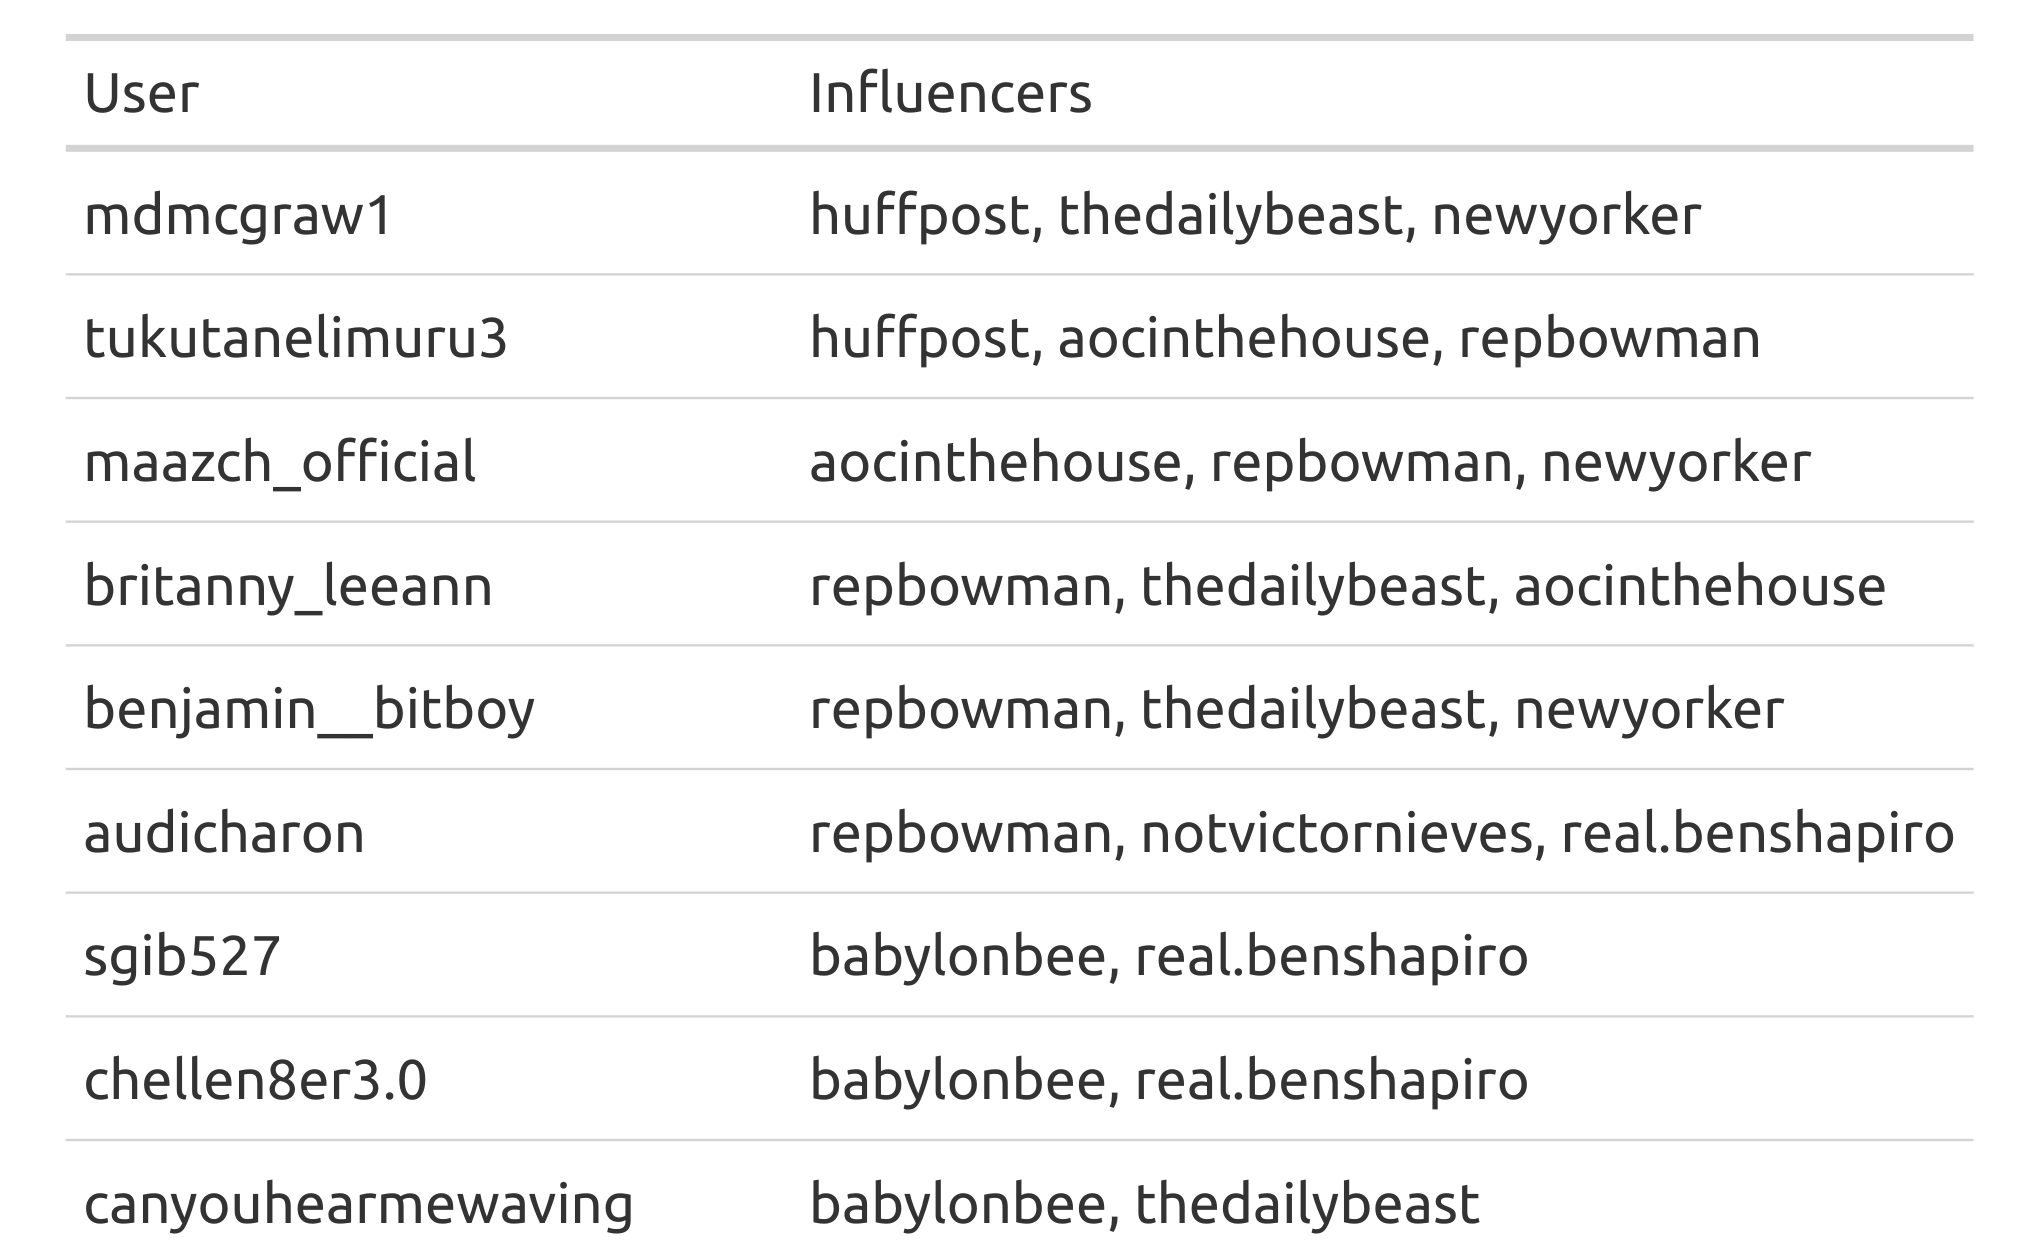
\includegraphics[width = .5\textwidth]{images/final_privacy_table.png}

As we can see, only six users follows more than three super-users and, generally speaking, most users follows super-users of the same political affiliation. Considering the scarcity of data, if a user follows less than 100\% of super-users from the same political spectrum, it is difficult to say anything about their political beliefs.

Let's make some examples: taken into consideration the table shown above (which is a small sample of the original, available a the following link: \url{https://github.com/albertomorini/CNS/blob/main/privacy_table.html}) we can say the following:

\begin{itemize}
    \item User \textit{mdmcgraw1} follows three super-users, all left-leaning, therefore is classified as left-leaning;
    \item User \textit{audicharon} follows three super-users, one left-leaning, two right-leaning, therefore nothing can be said about its political orientation;
    \item User \textit{chellen8er3.0} follows two super-users, both right-leaning, therefore is classified as right-leaning.
\end{itemize}

In future extensions, this classification could be improved by giving weights to super-users: \textit{repbowman} could weight more than \textit{notvictornieves} because the latter is an influencer, while the former is a politician.
\section{Engagement}

Studying engagement on TikTok can reveal how many people are reached and the approval rate of content.

Each post (in this case, only videos) includes several pieces of information that can be used to analyze the content's impact. For example, the API returns data such as the number of views, comments, likes, shares, and more.

Naturally, views have the highest numbers, followed by likes and comments. For these video topics, there is a very low "repost" rate (called shares), which refers to users reposting the influencer's video.

In the analysis, some attributes has been normalized thus to obtain a graph well formed.
In detail: views, likes, comments are reported in thousands

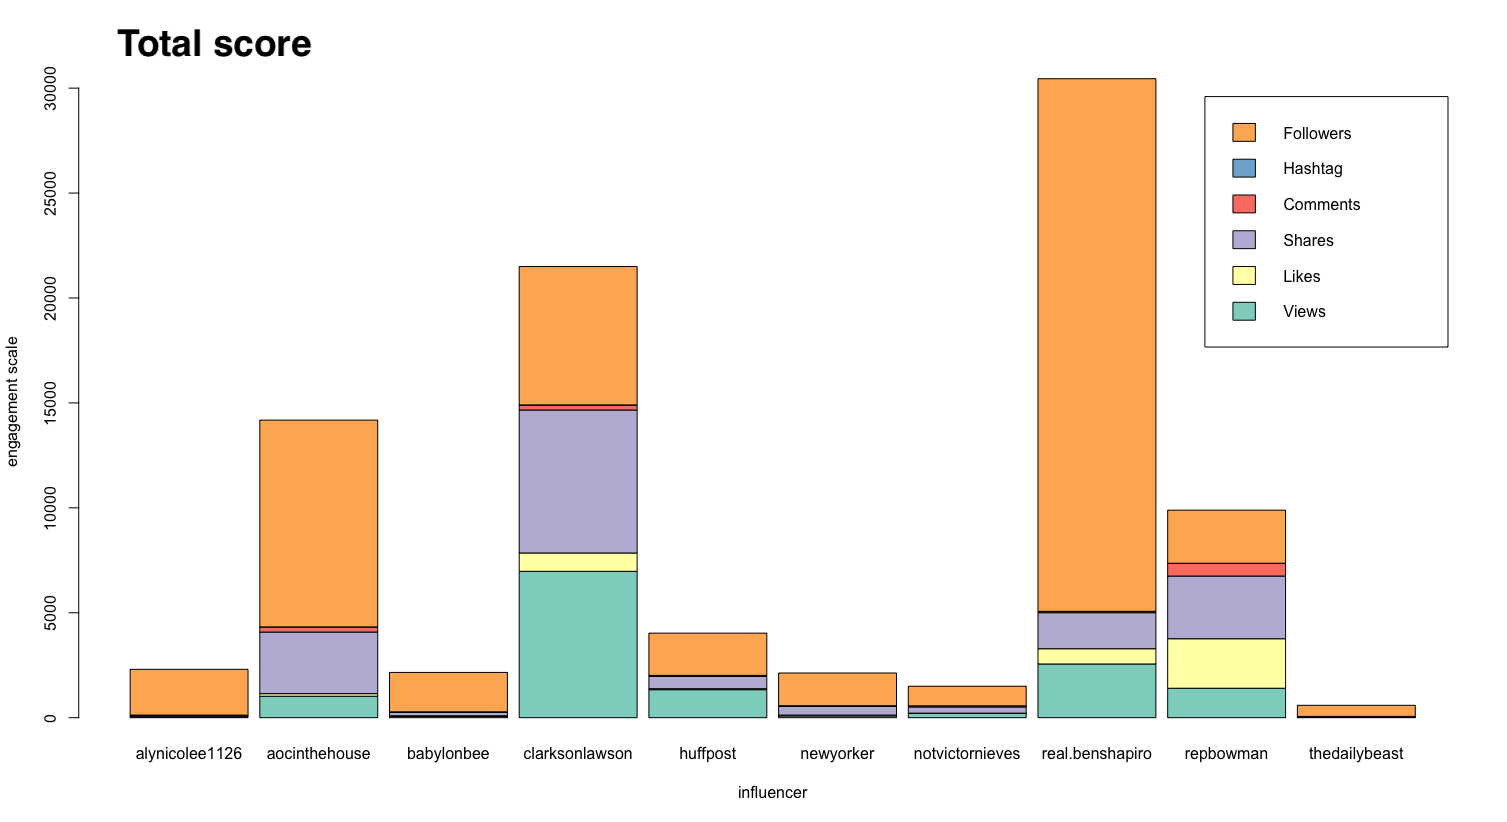
\includegraphics[width = .48\textwidth]{images/Final_Engagement_TotalScore.png}

To compare the two political wings, the data has been divided into two subgroups based on the side of influencers.

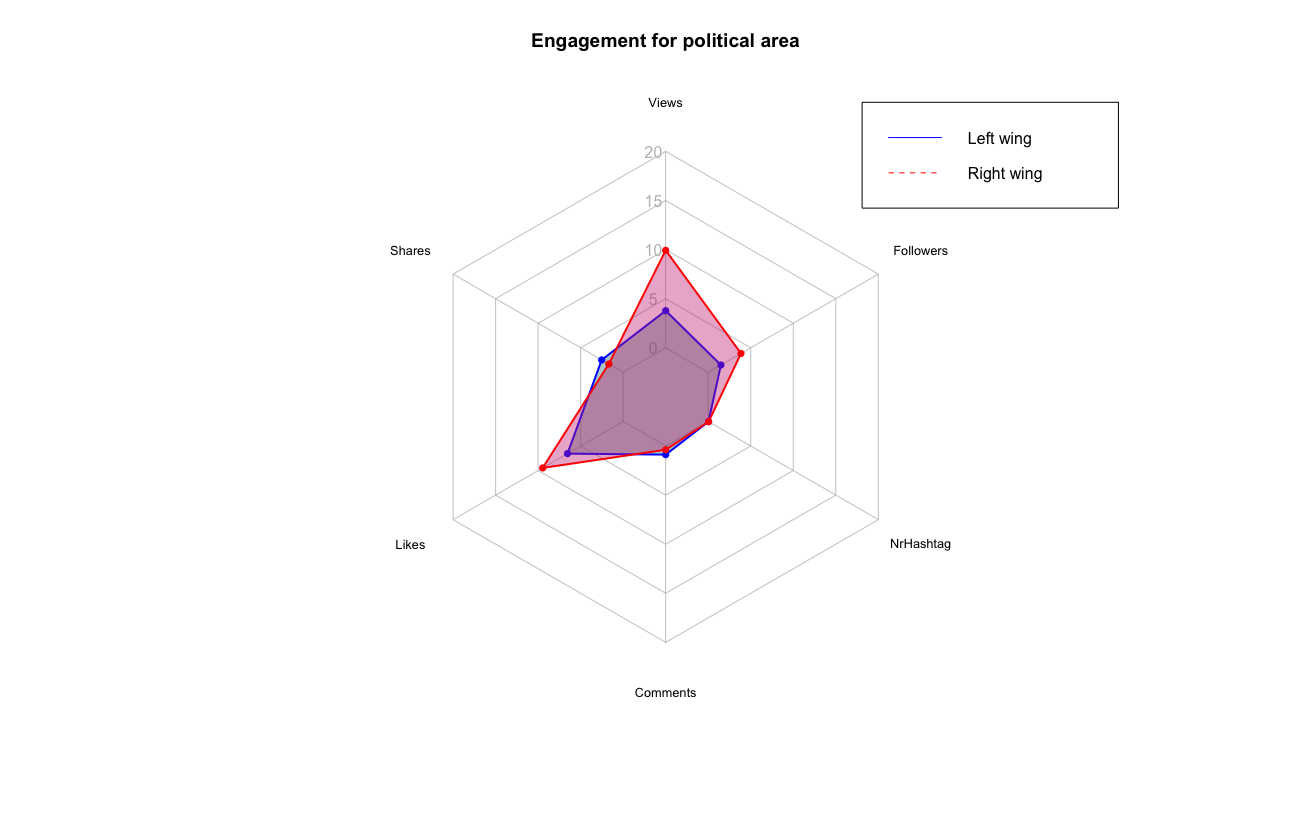
\includegraphics[width = .48\textwidth]{images/Final_Engagement_EngegementPerArea.png}
\section{Content Impact}

One aim of this research is to analyze the impact posting new content has on super-users' followers counts.

To this end, all videos posted by a super-user were downloaded over the span of five months. For each video, all new followers within five days from the upload date were registered.

\begin{lstlisting}[language=json]
{
    "data": {
        "cursor": 1717588518,
        "has_more": true,
        "user_followers": [
            {
                "username": "rev6luv",
                "display_name": "t."
            },
            {
                "display_name": "Caden M. Flanagan",
                "username": "therealcadenflanagan"
            },
            ...
    }
} 
\end{lstlisting}

There is a potential bias in this approach, as new followers can be gained independently of posted content. However, in the current social network landscape, content either goes viral almost immediately or not at all. For this reason, this approach has been considered valid.

The query included in the body of the request contains only the username, without filtering other parameters (such as hashtag, or region). This decision has been made since a super-user, while eclectic in the topics discussed, still belongs to a specific political orientation.

\begin{lstlisting}[language=json, label={lst:query}]
{
    "and": [
        {
            "operation": "IN",
            "field_name": "username",
            "field_values": [
                "$influencer" 
            ]
        }
    ]
}
\end{lstlisting}

In this analysis, only the most influential super-users have been considered (those with more followers and higher engagement values):

\begin{figure}[H]
    \centering
    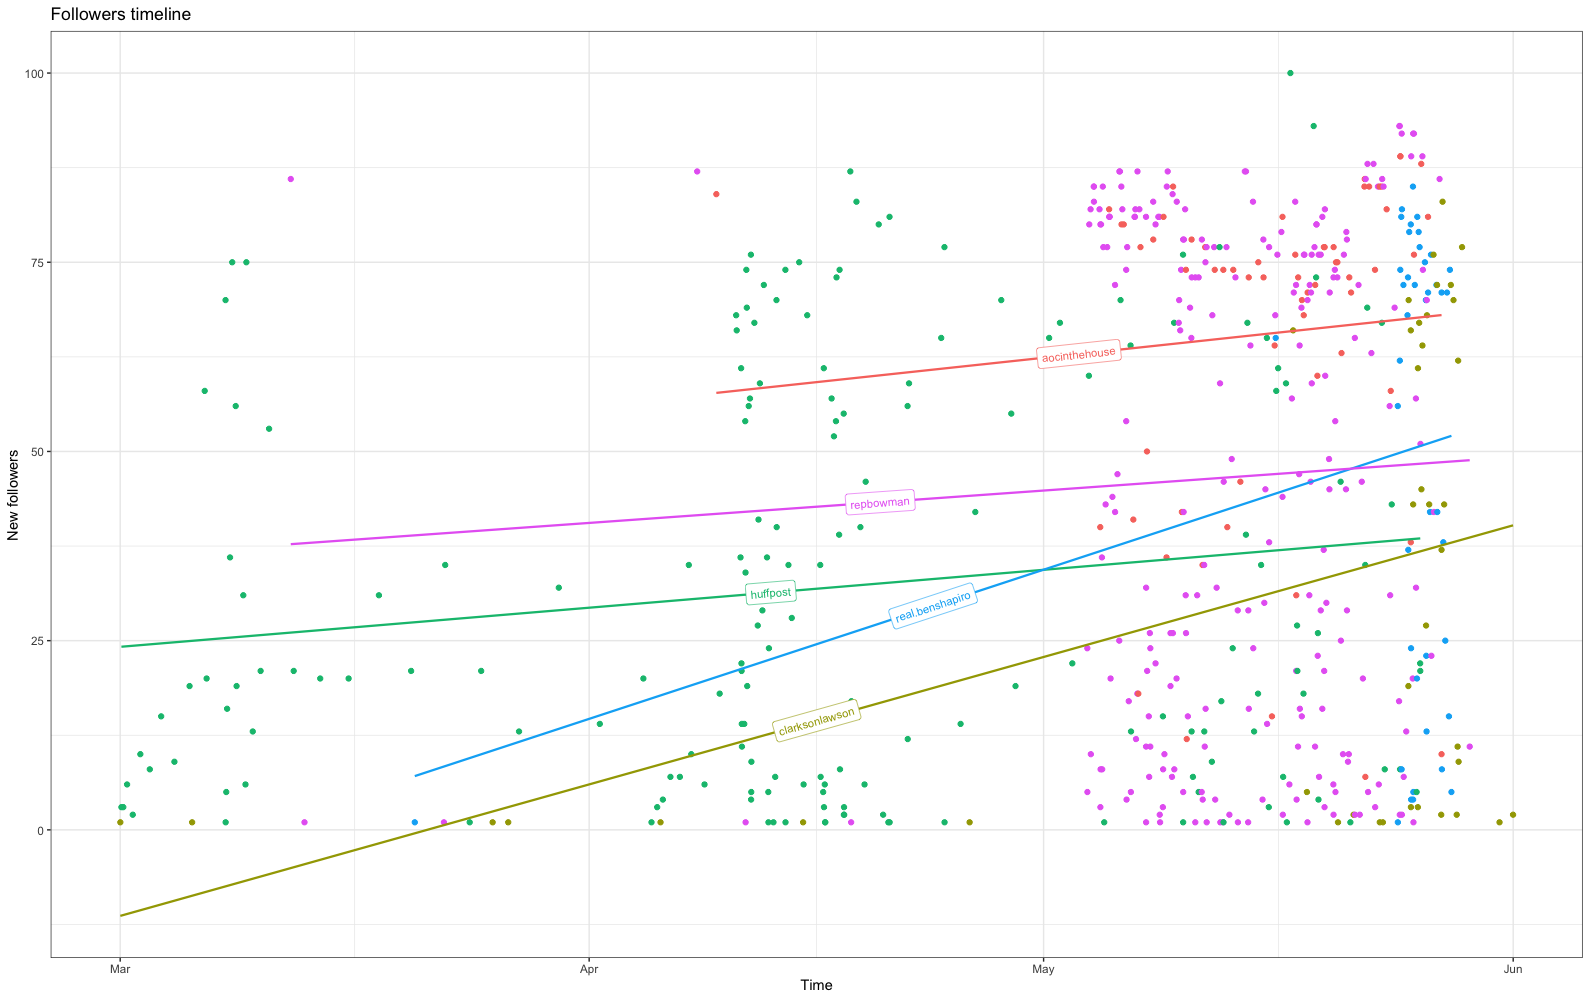
\includegraphics[width = .48\textwidth]{images/Final_Followers_Timeline.png}
    \caption*{As can be seen, the total number of followers increases steadily over time for almost all super-users.}
\end{figure}

A more specific analysis has been done on two super-users of particular interest: \textit{@aocinthehouse} and \textit{@real.benshapiro}:

\begin{figure}[H]
    \centering
    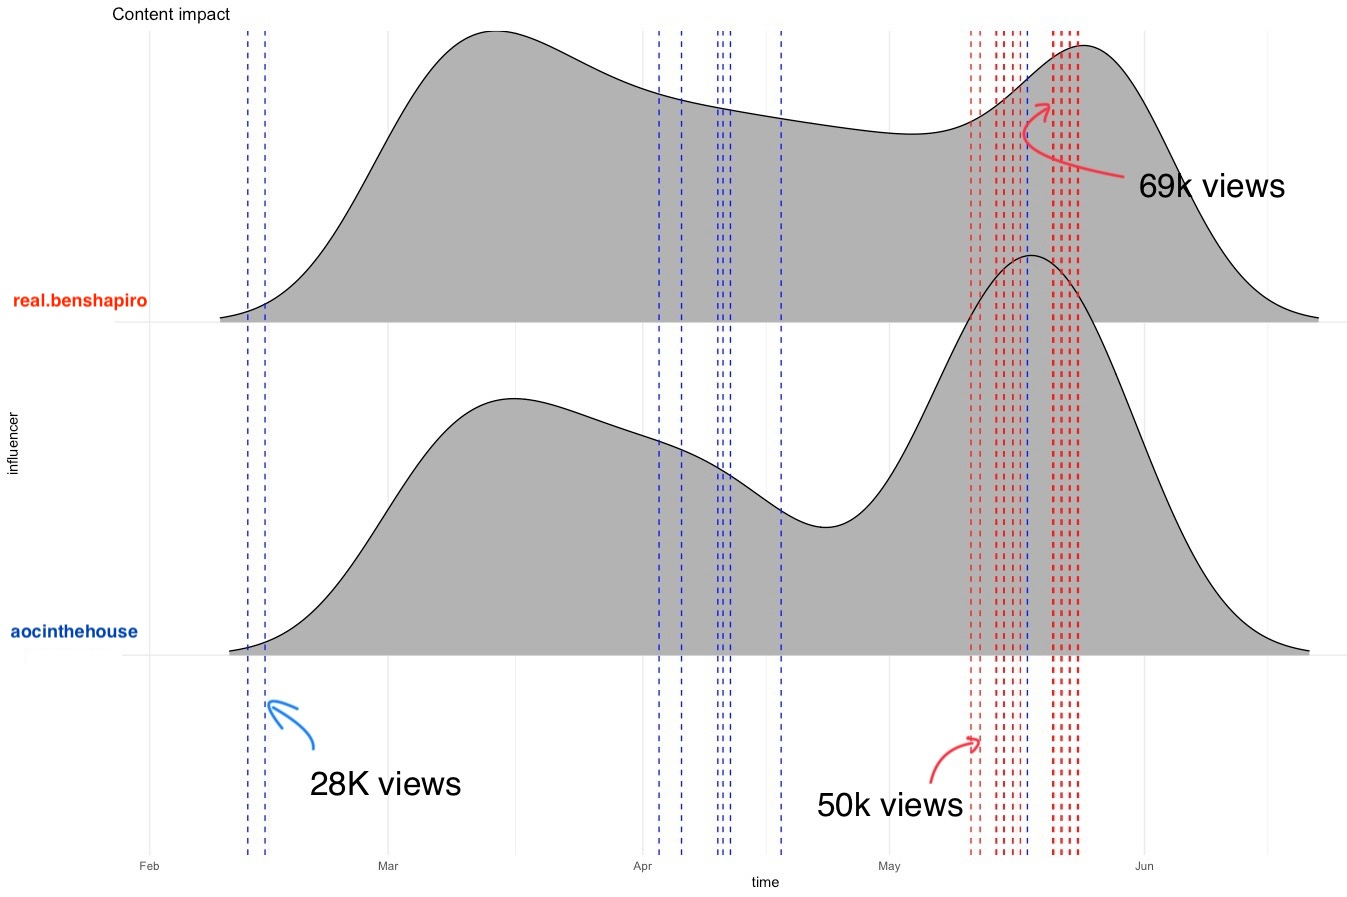
\includegraphics[width = .48\textwidth]{images/Final_ContentImpact_Custom.jpg}
    \caption*{This analysis consisted of the average trend of new followers, creating a detailed curve enriched with timestamps of new post creations.}
\end{figure}

In the graph shown above, there is a noticeable increase in new followers for \textit{@aocinthehouse} after the content posted on 15 February was viewed 28,000 times.

The aforementioned bias is evident in the increase in \textit{@real.benshapiro}'s follower count in mid-March despite not being active on TikTok. It can be inferred that influence on followers' count extends beyond TikTok, supported by the release of a YouTube video on 9 March 2024, which received nearly 300,000 views.

\section{Conclusions}

While gathering data through TikTok's official APIs has proven difficult, the amount of total information ultimately obtained was satisfying: 35,798 distinct followers and 182 videos were downloaded among 10 selected super-users.

This dataset was used to visualize the network and identify the presence of echo chambers (numerically confirmed by the low cosine similarity between super-users), measure users' engagement (revealing higher participation by right-leaning accounts), and to demonstrate the impact a posted video has on both engagement and the number of followers.

Finally the information was utilized to develop a prototype for inferring political orientation, although the high degree of isolation mentioned before made it difficult to draw clear conclusions.

All the source code can be found publicly at: \url{https://github.com/albertomorini/CNS}, while the data downloaded is kept secret to preserve the privacy of users.

\section{Extensions}

Regarding echo chambers, privacy inference, engagement, and content impact, better results could be achieved by significantly increasing the number of gathered data points. For example, one could circumvent the limitations imposed by TikTok's APIs by using third-party alternatives such as \url{https://github.com/davidteather/TikTok-Api}.

Another approach to enhance the social graph could involve collecting not only the super-users' followers but also the accounts they follow. This strategy, while powerful, would exponentially increase the number of data points, potentially making the processing phase rather computationally onerous.

Incorporating users' comments into the dataset would allow for sentiment analysis using large language models (LLMs), facilitating the study of polarization. These observations could be intersected with prior findings. Additionally, utilizing language recognition tools and analyzing users' pinned, shared, and liked videos (obtainable through official APIs) could help infer geo-location information, which would be valuable in our geopolitical context.
%%%%%%%%%%%%%%%%%%%%%%%%%%%%%%%%%%%%%%%%%
%             BIBLIOGRAPHY
%%%%%%%%%%%%%%%%%%%%%%%%%%%%%%%%%%%%%%%%%
\bibliographystyle{abbrv}
\bibliography{references}

\end{document}